\documentclass[openany]{article}


%Standard Stefanos Packages
\usepackage[utf8]{inputenc}
\usepackage{dirtytalk}
\usepackage{amsmath}
\usepackage{mathtools}  
\mathtoolsset{showonlyrefs} 
\usepackage{graphicx}
\usepackage{mdframed}
\usepackage{lipsum}
\usepackage{cancel}
\usepackage{systeme}
\usepackage{pgfplots}
\usepackage{textcomp}
\usepackage{amssymb}
\usepackage{geometry}
\usepackage{tikz-cd}
\usetikzlibrary{arrows}
\geometry{a4paper}
\graphicspath{ {./res/} }
\usepackage{float}
\restylefloat{table}
\newcommand{\comment}[1]{%
	\text{\phantom{(#1)}} \tag{#1}
}
 \title{\line(3,0){250}\\Artificial Intelligence \\ Genetic Algorithms Coursework  \\\line(3,0){250}}
\usepackage{pgfplots}
\newmdtheoremenv{note}{Note}
\newmdtheoremenv{definition}{Definition}
\pgfplotsset{compat=1.17}
%Extra Packages
\usepackage{tikz}
\usetikzlibrary{automata,positioning}

\usepackage{listings}
\usepackage{xcolor}

\definecolor{dkgreen}{rgb}{0,0.6,0}
\definecolor{gray}{rgb}{0.5,0.5,0.5}
\definecolor{mauve}{rgb}{0.58,0,0.82}
%Additional Packages
\usepackage{listings}
\usepackage{subcaption}
\lstdefinestyle{myScalastyle}{
	frame=tb,
	language=scala,
	aboveskip=3mm,
	belowskip=3mm,
	showstringspaces=false,
	columns=flexible,
	basicstyle={\small\ttfamily},
	numbers=none,
	numberstyle=\tiny\color{gray},
	keywordstyle=\color{blue},
	commentstyle=\color{dkgreen},
	stringstyle=\color{mauve},
	frame=single,
	breaklines=true,
	breakatwhitespace=true,
	tabsize=3,
}
\begin{document}
	\maketitle
	\pagebreak
	\section{Abstract}
		Lorem ipsum dolor sit amet, consectetur adipiscing elit. Phasellus vitae bibendum risus. Vestibulum mattis dui eros, 
		eu tristique orci egestas eu. Maecenas hendrerit mi eget nulla malesuada hendrerit. Praesent egestas dui eget ipsum fringilla, 
		vitae sagittis urna varius. In hac habitasse platea dictumst. In nec magna tellus. Nullam tempus rutrum lectus, nec ornare urna 
		posuere non. Praesent nec arcu tristique nisi elementum luctus nec quis lorem. Cras ullamcorper urna vitae volutpat euismod. Nunc 
		tincidunt lorem et augue interdum sodales. Quisque erat mi, viverra ut quam a, rutrum ornare mi. Donec eget sagittis metus. 
		Vestibulum ante ipsum primis in faucibus orci. 
	\pagebreak
	\section{Continous Optimisation}
		\begin{note}
			All the results for this section were produced with the following parameters.
			\begin{itemize}
				\item N=4
				\item Lower bound = -5
				\item Upper bound = 5
			\end{itemize}
			No further mentions will be provided for those hyperparameters.
		\end{note}
		\subsection{Subtask 1.C: Performance}
			For our algorithm evaluation, we will use two classic optimization testing functions, F1 and F4.
			\subsubsection{Sphrere}
				The Sphere(Commonly known as $F_{1}$ in the literature\cite{performance}) contains a single minimum and is considered an easily solvable function.
				\begin{equation}
				F_1(X)=\sum_{i=1}^{n}{x_{i}^2}
				\end{equation}
			\subsubsection{Rastrigin's function}
				Rastrigin’s function(Commonly known as $F_{4}$ in the literature\cite{performance}) is considered a challenging task due to its large number of local minima and its enormous search space.
				\begin{equation}
				F_4(X)=10\cdot n+\sum_{i=1}^{n}[x_{i}^{2}-10\cos(2\pi x_{i})]
				\end{equation}
			\subsubsection{Optimal hyperparameters}
				Before evaluating our algorithm's performance, we should first find the optimal hyperparameters for solving our test functions.
				We need to evaluate the following 3 variables and their affect on the algorithms performance.
				\begin{itemize}
					\item Mutation Rate(MR)
					\item Crossover Rate(CR)
					\item Population Size(PO)
				\end{itemize}
				We will use the following unbiased metric for measuring the objective performance for a given function($F_1$ or $F_4$) applied on the giver parameters (MR, CR, PO).
				\pagebreak
				\begin{definition}
					We define the following metric called 'Normalized Performance for function $F_{x}$'\footnote{We assume that the calculation of a single individual takes constant time (O(1))}
					\begin{equation}
						NF_{x}=1-\frac{g\cdot PO}{G\cdot max(PO)},\space 0\le NF_{x}\le 1
					\end{equation}
					Where the $g$ is the average number of generations untill the solution is found after 10 simulations, for a given MR,CR,PO on a given function $F_{x}$, $G$ is
					the maximum number of generations allowed and $max(PO)$\footnote{We multiply PO and max(PO) here, as can be proven that, without accounting the population size, our metric is biased} is the maximum population size allowed.
				\end{definition}
				\begin{figure}[H]
					\centering
					\begin{subfigure}{.5\textwidth}
						\centering
						\begin{center}
							\begin{figure}[H]
								\iftrue
								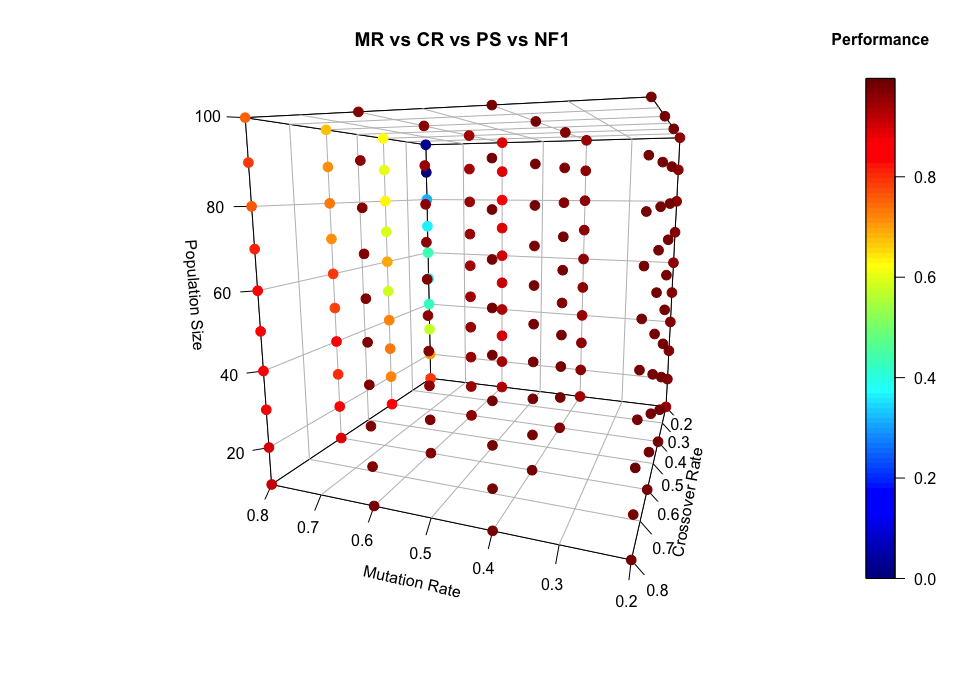
\includegraphics[scale=0.2]{res/hyperF1}
								\fi
							\end{figure}
						\end{center}
						\caption{Performance for $F_1$}
						\label{fig:sub1}
					\end{subfigure}%
					\begin{subfigure}{.5\textwidth}
						\centering
						\begin{center}
							\begin{figure}[H]
								\iftrue
								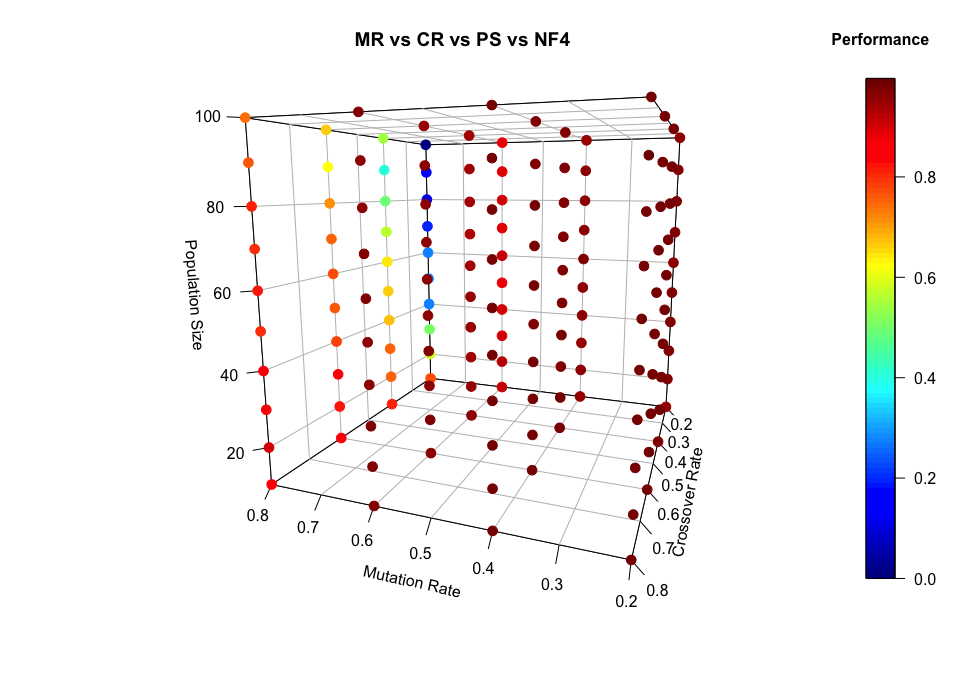
\includegraphics[scale=0.2]{res/hyperF4}
								\fi
							\end{figure}
						\end{center}
						\caption{Performance for $F_4$}
						\label{fig:sub2}
					\end{subfigure}
					\caption{Performance for 160 simulations per function}
					\label{fig:test}
				\end{figure}
				By visualizing the results, we can see that we get a very consistent performance by using the following hyperparameters.
				\begin{figure}[H]
					\centering
					\begin{center}
						\begin{tabular}{||c c c||} 
							\hline
							& Lower Bound & Higher Bound \\ [0.5ex] 
							\hline\hline
							MR & 0.2 & 0.4 \\ 
							\hline
							CR & 0.6 & 0.8 \\ 
							\hline
							PO & 80 & - \\ 
							\hline
						\end{tabular}
					\end{center}
					\caption{Optimal hyperparameters}
					\label{fig:sub1}
				\end{figure}
				\pagebreak
			\subsubsection{Performance Results}
				Using the optimal hyperparameters, as well as our optimal select and mutate operators (see \ref{tuning})
				\begin{figure}[H]
					\iftrue
					\centering
					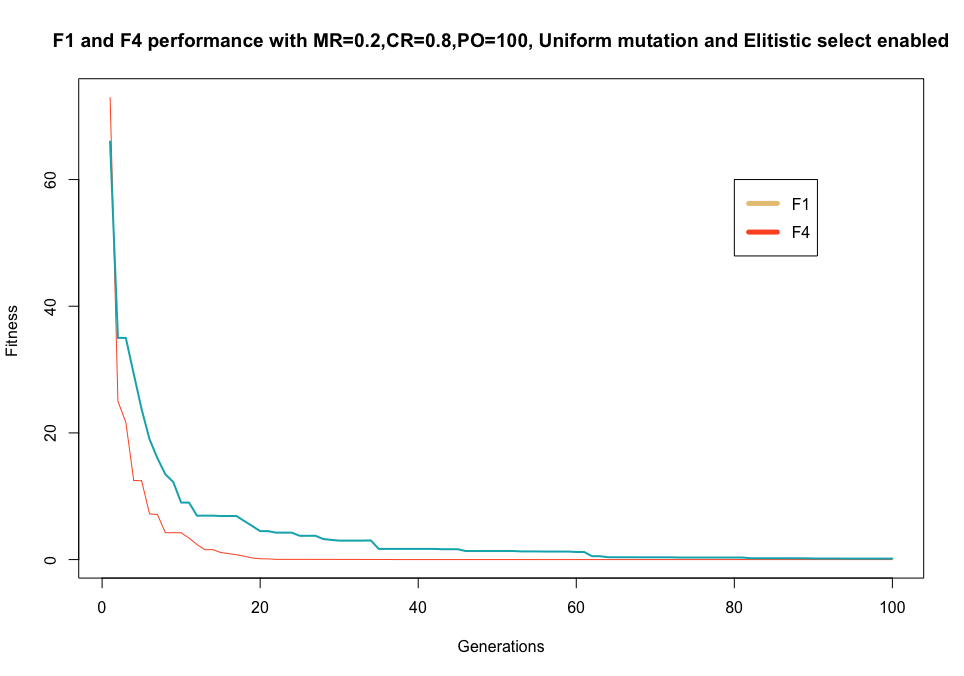
\includegraphics[scale=0.4]{res/perfF1F4}
					\fi
				\end{figure}
				We can see that the algorithm converges close enough to the global minima of each function in the first few generations, then it spends 
				the majority of its time oscillating around the desired result. This can be solved using more sophisticated mutation and crossover operators
				that are outside of the scope of this coursework.
				
				
				
				
				
				
		\subsection{Subtask 1.D, algorithm tuning}
			\label{tuning}
			The initial version of the algorithm was improved in the following 2 areas
			\begin{itemize}
				\item Balanced and Elitistic selection operator
				\item Mutation step distribution
			\end{itemize}
			\subsubsection{Balanced and Elitistic selection}
				The initial implementation of the selection operator involved a balanced wheel selection based on the relative fitness of the individual on the current generation, as well as
				an individual probability of each individual to mate. Using both metrics, we determined if an individual was allowed to mate or not. This implementation allowed less ideal
				candidates for mating with some probability, as this approach allowed the algorithm to avoid local minima traps efficiently. After some refinement, this approach was abandoned for a 
				more straightforward elitistic wheel selection. In this selection strategy, relative fitness is the only factor that affects an individual's probability to mate. The data below shows the 
				improvement using the more straightforward method.
				\subsubsection{Gaussian and Uniform mutation step}
				The mutation operator's initial implementation used a step taken from a Gaussian distribution with $\mu=0,\sigma=1$. 
				The desired effect was to select a tiny step as a mutation operation most of the time while leaving a small probability for a 
				more significant step to avoid local minima in case of a stuck. The performance analysis showed that the gaussian mutation operator
				was not 'wide' enough, and the algorithm spent an enormous time stuck on local minima. This was improved significantly by choosing 
				a uniform distribution within the range [-1,1]. As the probability for a more considerable step increases, the probability of 
				sticking into some local minima for too long decreases, and overall we can observe a performance gain as we reduce the number of
				generations to converge significantly
				\begin{figure}[H]
					\iftrue
					\centering
					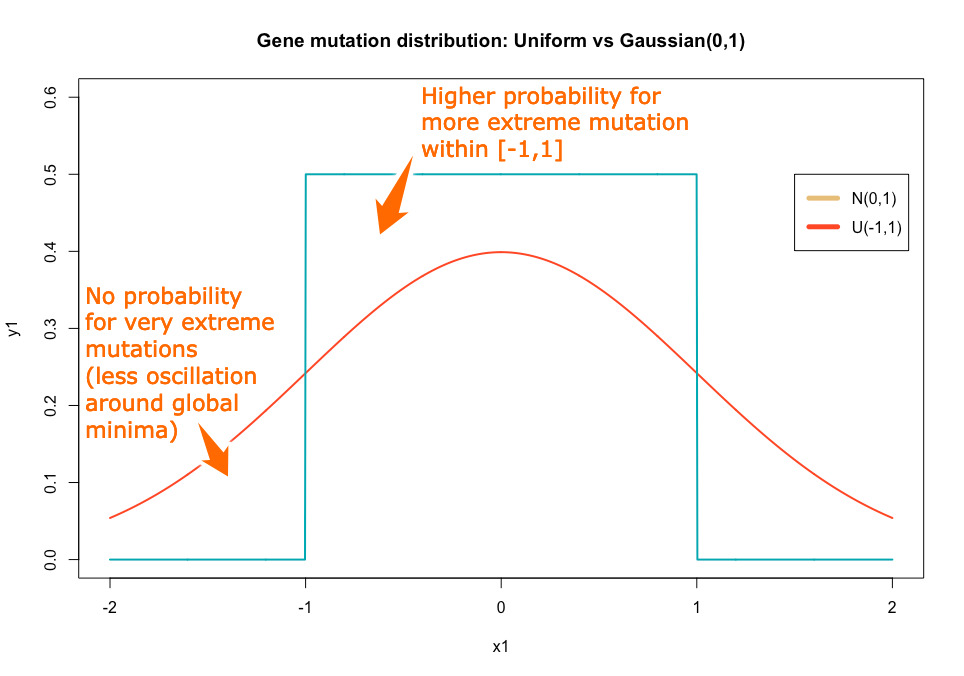
\includegraphics[scale=0.4]{res/geneMutation.jpeg}
					\fi
				\end{figure}	
				\begin{note}
					The following results was produced with the following hyperparameters
					\begin{itemize}
						\item Population 1000
						\item Crossover Rate 0.8
						\item Mutation Rate 0.2
					\end{itemize}
				\end{note}
				\begin{figure}[H]
					\centering
					\begin{subfigure}{.5\textwidth}
						\centering
						\begin{center}
							\begin{tabular}{||c c c||} 
								\hline
								  & Balanced & Elitistic \\ [0.5ex] 
								\hline\hline
								F1 & 124 & 98 \\ 
								\hline
								F4 & 107 & 87 \\
								\hline
							\end{tabular}
						\end{center}
						\caption{Balanced vs Elitistic(Gaussian Mutation)}
						\label{fig:sub1}
					\end{subfigure}%
					\begin{subfigure}{.5\textwidth}
						\centering
						\begin{center}
							\begin{tabular}{||c c c||} 
								\hline
								& Balanced & Elitistic \\ [0.5ex] 
								\hline\hline
								F1 & 133 & 90 \\ 
								\hline
								F4 & 94 & 67 \\
								\hline
							\end{tabular}
						\end{center}
						\caption{Balanced vs Elitistic(Uniform Mutation)}
						\label{fig:sub2}
					
					\end{subfigure}
					\begin{subfigure}{.5\textwidth}
						\centering
						\begin{center}
							\begin{tabular}{||c c c||} 
								\hline
								& Balanced Gaussian & Elitistic Uniform \\ [0.5ex] 
								\hline\hline
								$F_1$ & -6\% & +8\% \\ 
								\hline
								$F_4$ & +12\% & +22\% \\
								\hline
							\end{tabular}
						\end{center}
						\caption{Performance differences between the methods}
						\label{fig:sub2}
					\end{subfigure}
					
					\caption{Performance results on 10-Round averages}
					\label{fig:test}
				\end{figure}
				

		
		
		
\begin{thebibliography}{1}	
	\bibitem{wheel-selection}
	\textit{Bäck, Thomas, Evolutionary Algorithms in Theory and Practice (1996), p. 120, Oxford Univ. Press}
	
	\bibitem{holland-1975}
	\textit{Holland J.H. (1984) Genetic Algorithms and Adaptation. In: Selfridge O.G., Rissland E.L., Arbib M.A. (eds) Adaptive Control of Ill-Defined Systems. NATO Conference Series (II Systems Science), vol 16. Springer, Boston, MA. https://doi.org/10.1007/978-1-4684-8941-5\_21}
	
	\bibitem{performance}
	\textit{Carvalho, D. B. et al. “The Simple Genetic Algorithm Performance: A Comparative Study on the Operators Combination.” (2011).}
	
\end{thebibliography}
			
\end{document}